\documentclass[]{article}

% Imported Packages
%------------------------------------------------------------------------------
\usepackage{amssymb}
\usepackage{amstext}
\usepackage{amsthm}
\usepackage{amsmath}
\usepackage{enumerate}
\usepackage{extarrows}
\usepackage{fancyhdr}
\usepackage{float}
\usepackage[margin=1in]{geometry}
\usepackage{graphicx}
\usepackage{indentfirst}
\usepackage{setspace}
\usepackage{tikz}
%------------------------------------------------------------------------------

% Header and Footer
%------------------------------------------------------------------------------
\pagestyle{plain}  
\renewcommand\headrulewidth{0.4pt}                                      
\renewcommand\footrulewidth{0.4pt}                                    
%------------------------------------------------------------------------------

% Title Details
%------------------------------------------------------------------------------
\title{Deliverable \#3}
\author{SE 3A04: Software Design II -- Large System Design}
\date{\today}                               
%------------------------------------------------------------------------------

% Document
%------------------------------------------------------------------------------
\begin{document}

\maketitle	

\section{Introduction}
\label{sec:introduction}
% Begin Section
\subsection{Purpose}
\label{sub:purpose}
% Begin SubSection
% \begin{enumerate}[a)]
% 	\item Delineate the purpose of the document
% 	\item Specify the intended audience for the document
% \end{enumerate}
This document provides a detailed description of each the components and their operations. The interactions and relationships between components are also detailed in this document. The intended audience for this document is software engineers designing this system.
% End SubSection

\subsection{System Description}
\label{sub:system_description}
Ship Wreck is a single-player game with one core goal. This core goal is accomplished through playing five different mini-games. If the player fails to successfully finish a mini-game, the ship's health will be reduced. If the ship's health reaches or goes below 0, the ship is considered destroyed. As such, the player must successfully complete as many mini-games as provided during the ship's journey to ensure that the ship can reach its destination without being destroyed. Once the ship successfully arrives at its destination, the player wins.
% End SubSection

\subsection{Overview}
\label{sub:overview}
The rest of this document is organized into sections detailing the state charts of each controller class, sequence diagrams for each use case of the game, and a class diagram for the game.
% End SubSection

% End Section

\newpage
\section{State Charts for Controller Classes}
\label{sec:state_charts_for_controller_classes}
% Begin Section
This section should provide a state chart for each controller class for your application.
\begin{figure}[h]
    \centering
    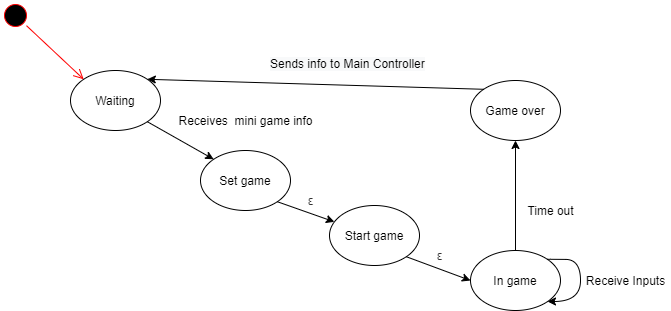
\includegraphics[width=\textwidth]{stateCharts/minigameSC.png}
    \caption{State Chart of Mini Game Controller}
\end{figure}

\begin{figure}[H]
    \centering
    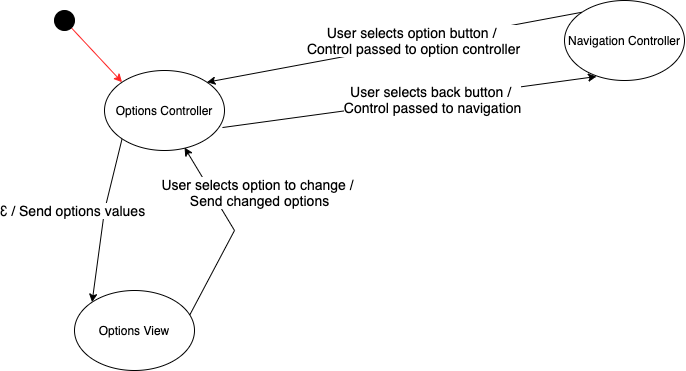
\includegraphics[width=\textwidth]{stateCharts/options_controller.png}
    \caption{State Chart of Option Controller}
\end{figure}

\begin{figure}[H]
    \centering
    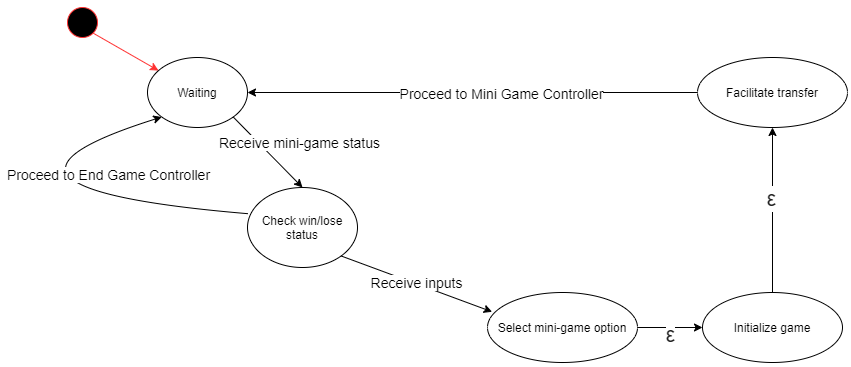
\includegraphics[width=1.0\textwidth]{stateCharts/mainhub_controller.png}
    \caption{State Chart of Main Hub Controller}
\end{figure}

\begin{figure}[H]
    \centering
    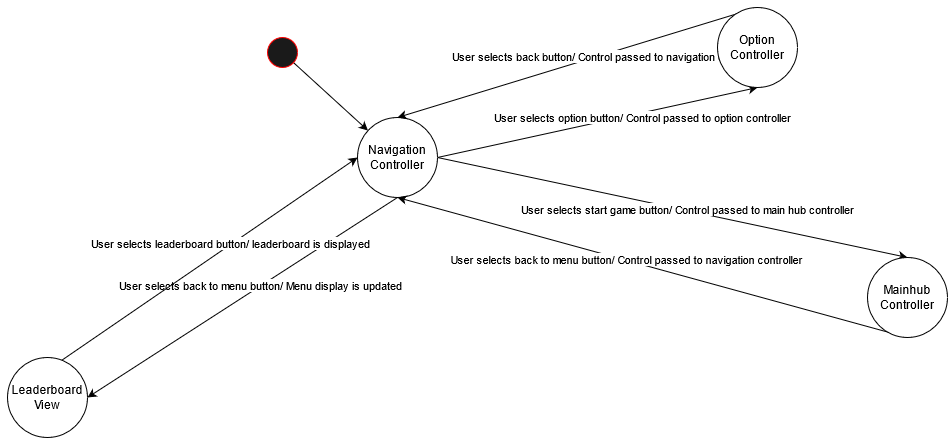
\includegraphics[width=\textwidth]{D3/stateCharts/statediagramnav.png}
    \caption{State Chart of Navigation Controller}
\end{figure}

\begin{figure}[H]
    \centering
    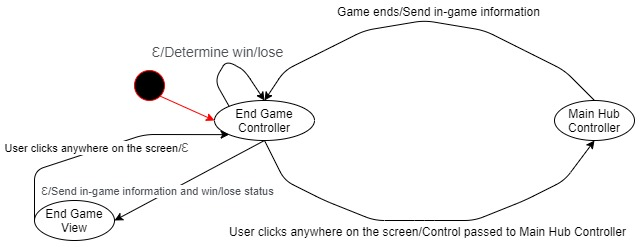
\includegraphics[width=\textwidth]{D3/stateCharts/end_game_state_chart.jpg}
    \caption{State Chart of End Game Controller}
\end{figure}
% End Section

\newpage
\section{Sequence Diagrams}
\label{sec:sequence_diagrams}
% Begin Section
This section should provide a sequence diagram for each use case of your application.

\begin{figure}[H]
    \centering
    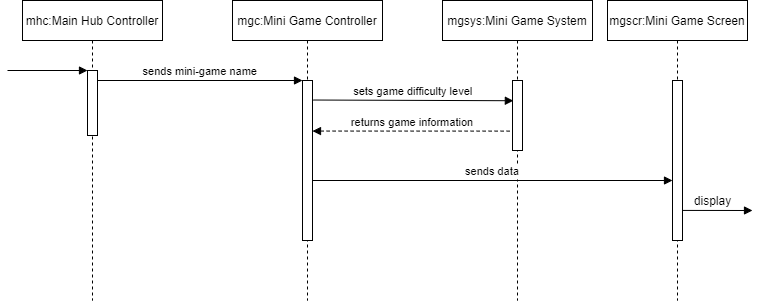
\includegraphics[width=\textwidth]{sequenceDiagrams/start_game.png}
    \caption{Use case: Start game}
    \label{fig:seq_start_game}
\end{figure}

\begin{figure}[H]
    \centering
    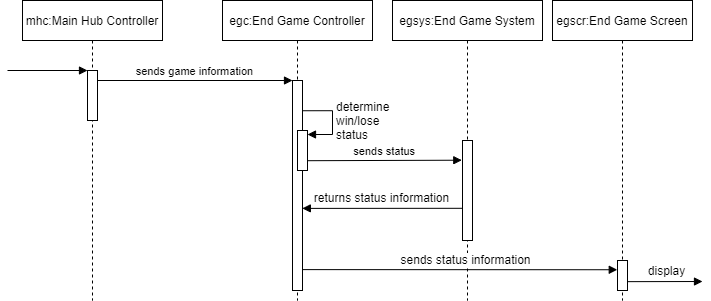
\includegraphics[width=\textwidth]{sequenceDiagrams/end_game.png}
    \caption{Use case: End game}
    \label{fig:seq_end_game}
\end{figure}

\begin{figure}[H]
    \centering
    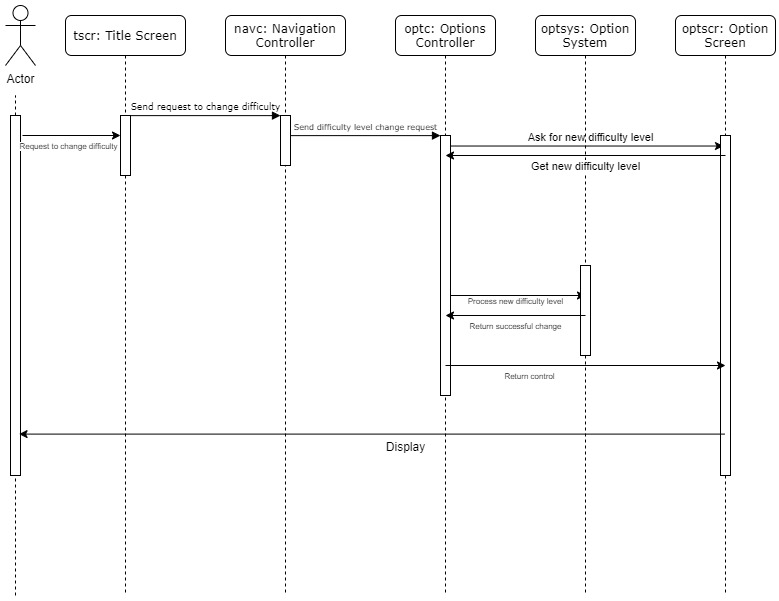
\includegraphics[width=\textwidth]{D3/sequenceDiagrams/change_diff.jpg}
    \caption{Use case: Change difficulty}
    \label{fig:seq_change_diff}
\end{figure}

\begin{figure}[H]
    \centering
    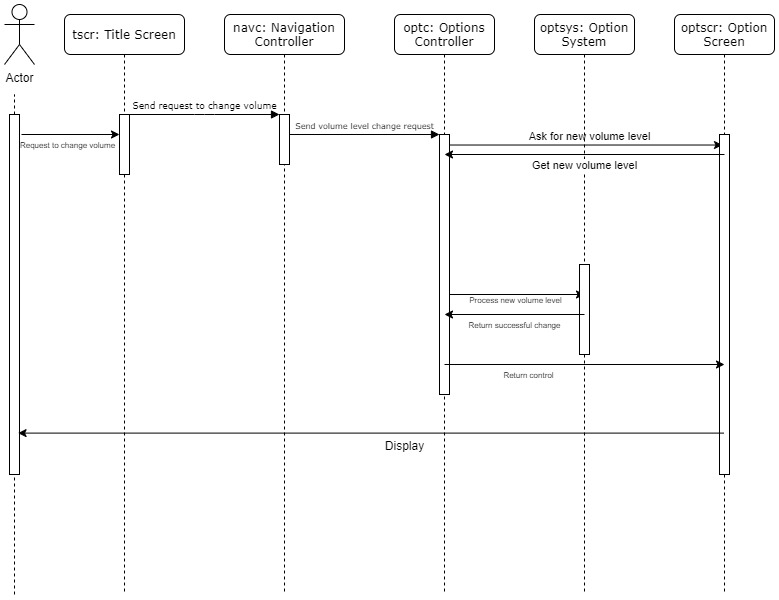
\includegraphics[width=0.9\textwidth]{D3/sequenceDiagrams/change_vol.jpg}
    \caption{Use case: Change volume}
    \label{fig:seq_change_vol}
\end{figure}

\begin{figure}[H]
    \centering
    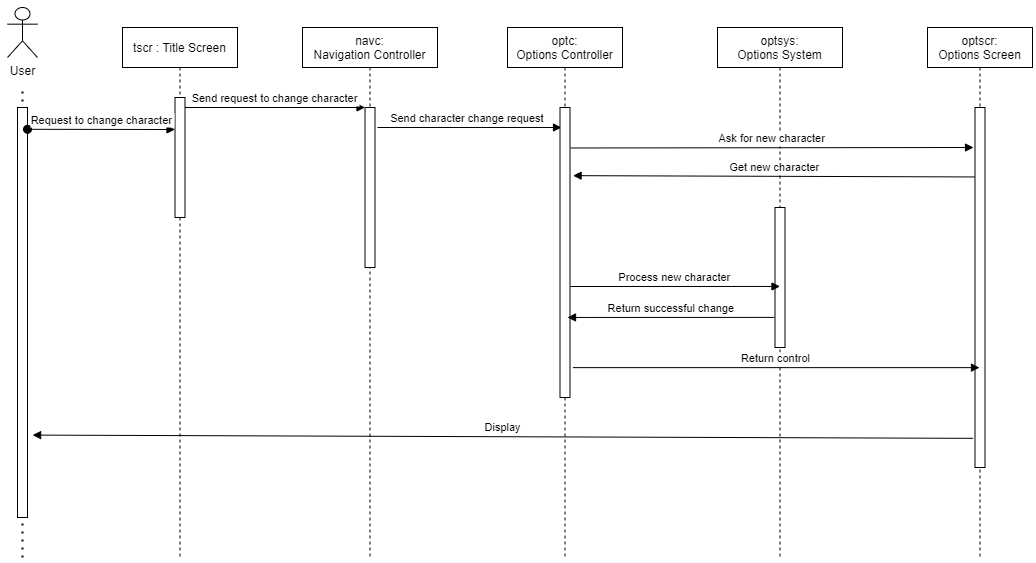
\includegraphics[width=0.9\textwidth]{D3/sequenceDiagrams/change_character.png}
    \caption{Use case: Change character}
    \label{fig:seq_change_char}
\end{figure}

\begin{figure}[H]
    \centering
    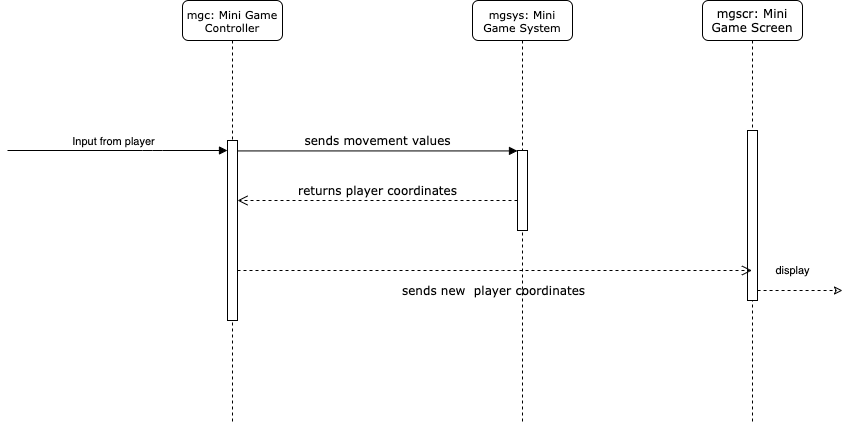
\includegraphics[width=0.9\textwidth]{D3/sequenceDiagrams/move_character.png}
    \caption{Use case: Move character}
    \label{fig:seq_move_char}
\end{figure}

\begin{figure}[H]
    \centering
    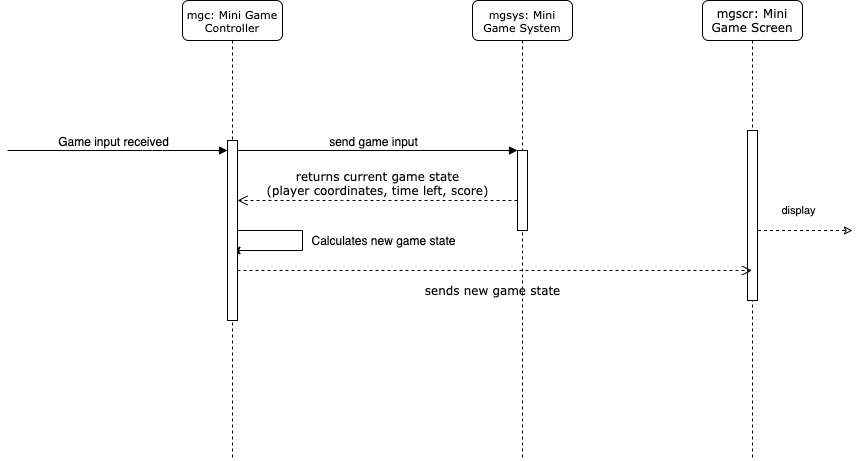
\includegraphics[width=0.9\textwidth]{D3/sequenceDiagrams/play_minigame.png}
    \caption{Use case: Play mini-game}
    \label{fig:seq_play_game}
\end{figure}

% End Section

\section{Detailed Class Diagram}
\label{sec:detailed_class_diagram}
% Begin Section
\begin{figure}[H]
    \centering
    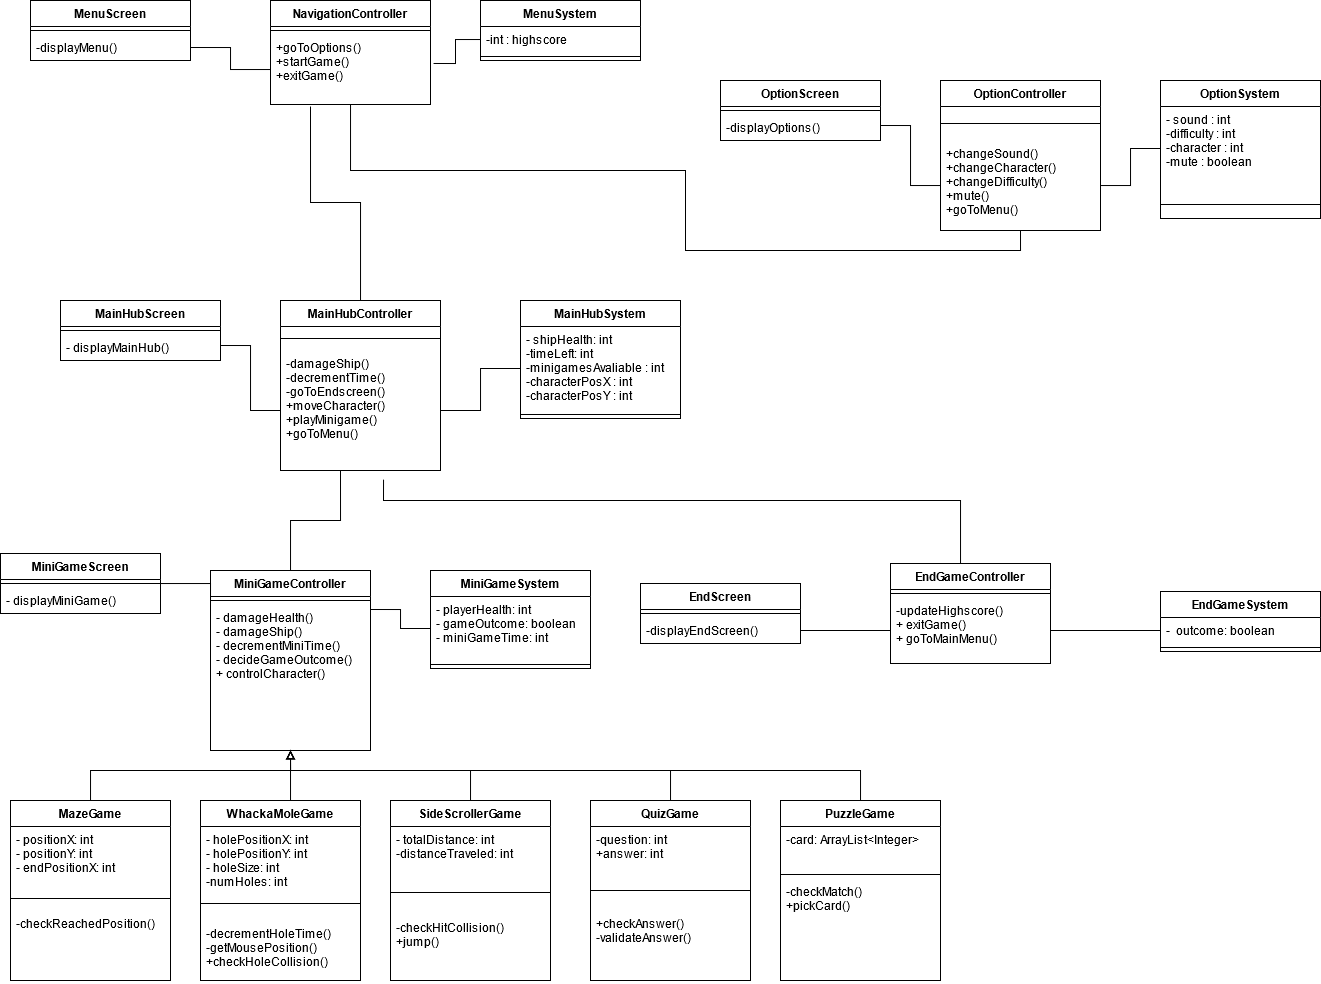
\includegraphics[width=0.9\textwidth]{D3/designdiagram/detailedclassdiagrams.png}
    \caption{Detailed Class Diagram}
    \label{fig:dcd}
\end{figure}

% End Section

\newpage
\appendix
\section{Division of Labour}
\label{sec:division_of_labour}
% Begin Section
Include a Division of Labour sheet which indicates the contributions of each team member. This sheet must be signed by all team members.

\begin{table}[h]
    \centering
    \begin{tabular}{|c|c|c|}
    \hline
        \textbf{Name} & \textbf{Contributed Part} & \textbf{Signature} \\
        \hline
        Benson & Section 1, Section 2 Figure 5, Section 3 Figure 8 \& 9
        & 
\includegraphics[width=0.3\textwidth]{signatures/bensonsignature.JPG}\\
        \hline
        Graeme &  Section 1, Section 2 Figure 2, Section 3 Figure 11 \& 12
        & 
\includegraphics[width=0.25\textwidth]{signatures/graeme_signature.png} \\
        \hline
        Jiawei & Section 1, Section 2 Figure 1, Section 3 Figure 6 \& 7
        & 
\includegraphics[width=0.3\textwidth]{signatures/Signature_Jiawei.PNG}\\
        \hline
        Nick & Section 1, Section 2 Figure 4, Section 4
        & 
\includegraphics[width=0.3\textwidth]{signatures/nick signature.PNG} \\
        \hline
        Rupinder & Section 1, Section 2 Figure 3, Section 3 Figure 10
        & 
\includegraphics[width=0.3\textwidth]{signatures/Rupinder Signature.png}\\
        \hline
    \end{tabular}
    \caption{Division of Labour}
    \label{tab:my_label}
\end{table}

% End Section

\newpage
\section*{IMPORTANT NOTES}
\begin{itemize}
	\item You do \underline{NOT} need to provide a text explanation of each diagram; the diagram should speak for itself
	\item Please document any non-standard notations that you may have used
	\begin{itemize}
		\item \emph{Rule of Thumb}: if you feel there is any doubt surrounding the meaning of your notations, document them
	\end{itemize}
	\item Some diagrams may be difficult to fit into one page
	\begin{itemize}
		\item It is OK if the text is small but please ensure that it is readable when printed
		\item If you need to break a diagram onto multiple pages, please adopt a system of doing so and thoroughly explain how it can be reconnected from one page to the next; if you are unsure about this, please ask me
	\end{itemize}
	\item Please submit the latest version of Deliverable 1 and Deliverable 2 with Deliverable 3
	\begin{itemize}
		\item They do not have to be a freshly printed versions; the latest marked versions are OK
	\end{itemize}
	\item If you do \underline{NOT} have a Division of Labour sheet, your deliverable will \underline{NOT} be marked
\end{itemize}


\end{document}
%------------------------------------------------------------------------------